\documentclass{article}

\usepackage{graphicx} % Required for inserting images
\usepackage[margin=1.2in]{geometry}
\usepackage{float}

\title{Control for CUSF}
\author{Yoonjae Hwang}
\date{Michaelmas 2025}

\begin{document}


\maketitle

\section{Modelling}
\begin{figure}[H]
\begin{center}
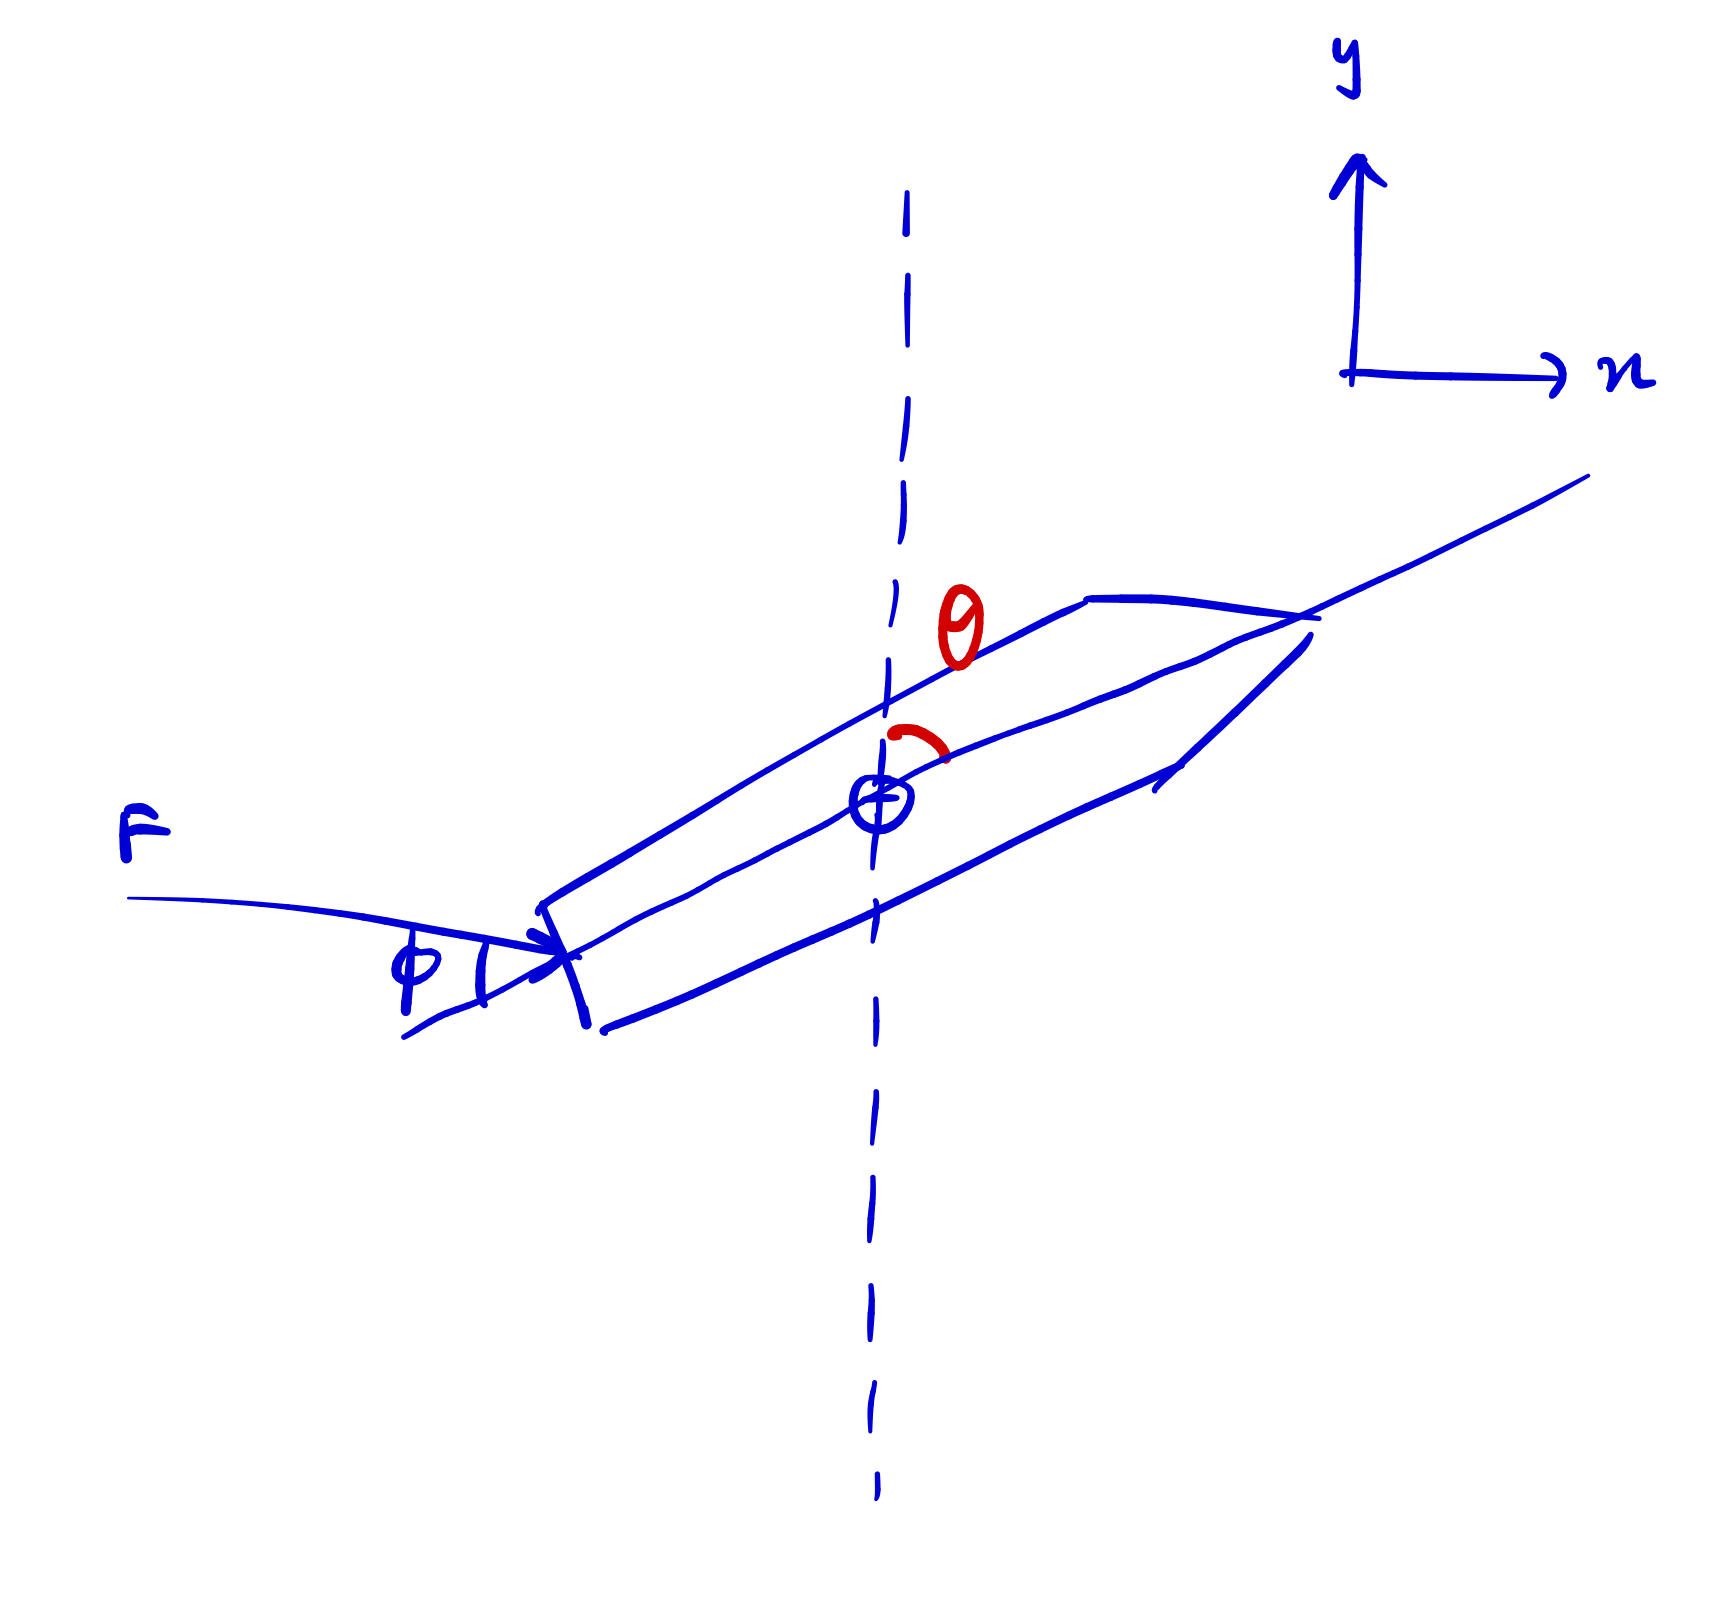
\includegraphics[width = 0.7\textwidth]{thumbnail_Image.png}
\caption{3DOF Thrust Vector Controlled Rocket}
\end{center}
\end{figure}

\begin{enumerate}
    \item Consider a 3DOF thrust vector controlled rocket, shown in figure 1. Write the equations of motion.
    \item Write the equations of motion in nonlinear state space form. 
    \item Write a function in MATLAB to implement this differential equation. The inputs should be the state $(x, y, \theta, \dot{x}, \dot{y}, \dot{\theta})$ and the inputs $(F, \phi)$. 
    \item For suitable initial conditions, try to predict what would happen analytically/intuitively and verify your simulation. 
\end{enumerate}

\section{Controller Design}
\begin{enumerate}
    \item Using the 'jacobian(f,x)' function in MATLAB, find the Jacobian of the nonlinear differential equation with respect to $\mathbf{x} = \left[ x, y, \theta,  \dot{x}, \dot{y}, \dot{\theta} \right]^{\top}$ and input $\mathbf{u} = \left[F, \phi \right]$.
    \item Substitute in the right parameters (there's a function for this too) and compute the 'A' and 'B' matrices to form a linear state space equation. 
    \item Define your state space system.
    \item Compute the controllability matrix, using the 'ctrb(A, B)' function. Check if the row rank condition is satisfied to verify that the system is reachable/controllable locally. 
    \item Identify where you might want your poles - this may take some trial and error, and use the 'place(A, B, p)' function to compute the gain matrix K for $\mathbf{u} = -\mathbf{K} \mathbf{x}$.
    \item Create a closed loop Simulink block diagram for this and run the simulation. 
\end{enumerate}


\end{document}
